\documentclass[14pt,a4paper]{article}
\usepackage[spanish,es-nodecimaldot]{babel}	% Utilizar español
\usepackage[utf8]{inputenc}					% Caracteres UTF-8
\usepackage{graphicx}						% Imagenes
\usepackage[hidelinks]{hyperref}			% Poner enlaces sin marcarlos en rojo
\usepackage{fancyhdr}						% Modificar encabezados y pies de pagina
\usepackage{float}							% Insertar figuras
\usepackage[textwidth=390pt]{geometry}		% Anchura de la pagina
\usepackage[nottoc]{tocbibind}				% Referencias (no incluir num pagina indice en Indice)
\usepackage{enumitem}						% Permitir enumerate con distintos simbolos
\usepackage[T1]{fontenc}					% Usar textsc en sections
\usepackage{amsmath}						% Símbolos matemáticos

\usepackage[table,xcdraw]{xcolor}
\setlength\headheight{26pt} 
\pagestyle{fancy}
\rhead{
\includegraphics[width=1cm]{./images/logo.png}}

% Comandos para poner el nombre de la asignatura
\newcommand{\asignatura}{Programación Lúdica}
\newcommand{\autor}{Carlos Nuñez Molina \\ Ignacio Vellido Expósito}
\newcommand{\titulo}{SynVic}
\newcommand{\subtitulo}{Manual de juego}

\begin{document}
    \pagenumbering{gobble}
    
% ==============================================================================
% Pagina de titulo
\begin{titlepage}
    \begin{minipage}{\textwidth}
        \centering

        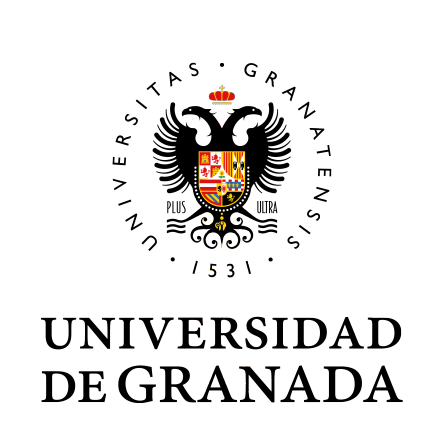
\includegraphics[scale=0.5]{images/ugr.png}\\

        \textsc{\Large \asignatura{}\\[0.2cm]}
        \textsc{GRADO EN INGENIERÍA INFORMÁTICA}\\[1cm]

        \noindent\rule[-1ex]{\textwidth}{1pt}\\[1.5ex]
        \textsc{{\Huge \titulo\\[0.5ex]}}
        \textsc{{\Large \subtitulo\\}}
        \noindent\rule[-1ex]{\textwidth}{2pt}\\[2.5ex]

        \end{minipage}

        \vspace{0.3cm}

        \begin{minipage}{\textwidth}

        \centering

        \textbf{Autores}\\ {\autor{}}\\[1.5ex]
        \vspace{0.2cm}

        
\includegraphics[scale=0.3]{images/etsiit.jpeg}

        \vspace{0.7cm}
        \textsc{Escuela Técnica Superior de Ingenierías Informática y de Telecomunicación}\\
        \vspace{1cm}
        \textsc{Curso 2019-2020}
    \end{minipage}
\end{titlepage}

% ==============================================================================
% ==============================================================================
    
    \pagenumbering{arabic}
    \tableofcontents
    \thispagestyle{empty}				% No usar estilo en la pagina de indice
    \newpage

    % ==============================================================================

    \section{Introducción}

SynVic es un MOBA 2v2 donde debes formar equipo con jugadores desconocidos y explotar al máximo las sinergias entre vuestros personajes para conseguir la victoria. SynVic es un juego en el que prima la cooperación y la adaptabilidad, y donde los jugadores eligen su personaje sin saber cuál será el objetivo ni quiénes serán el resto de personajes.
	\vspace{\baselineskip}
\vspace{\baselineskip}

\section{Controles}
El juego usa un sistema de control por teclado y ratón. Mediante clicks derechos del ratón se mueve al personaje por el mapa. Si se cliquea sobre un enemigo, el personaje aplicará un ataque básico sobre este.
Las teclas Q W E activan las tres habilidades básicas y la tecla R la habilidad definitiva.

\vspace{\baselineskip}

La cámara del jugador tiene dos modos: \emph{auto} y \emph{manual}. En modo \emph{auto}, la cámara sigue el movimiento del jugador y siempre está centrada sobre este. En modo \emph{manual}, la cámara está fija y no sigue al jugador. En este modo, la cámara se desplaza arrastrando el ratón hacia los bordes de la pantalla. Al pulsar la tecla \emph{Space}, se cambia entre un modo y otro.

\vspace{\baselineskip}

\begin{figure}[h]
	\centering
	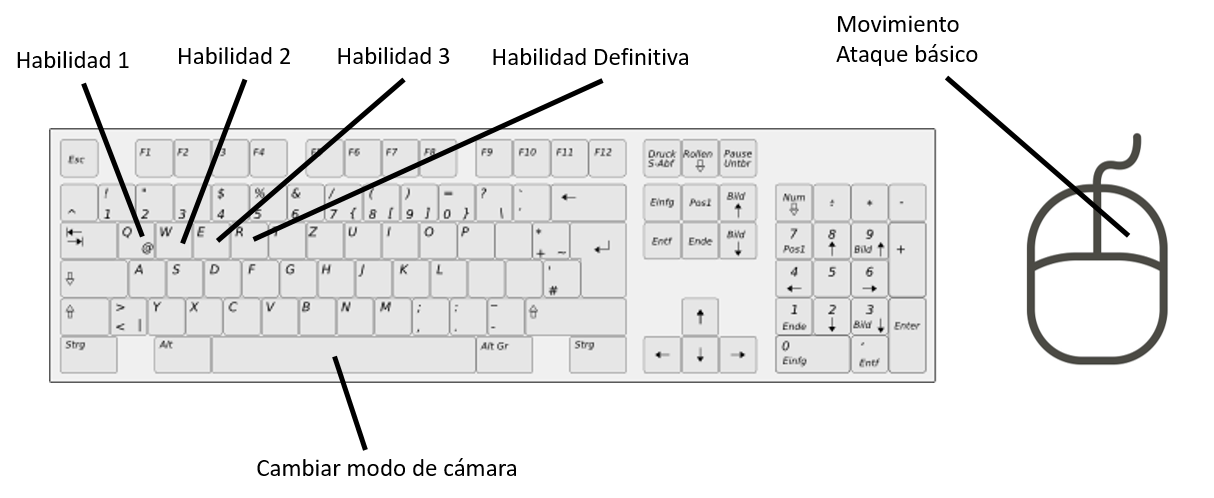
\includegraphics[width=0.8\linewidth]{figures/controles.png}
	% \caption{Controles}
\end{figure}

% ==============================================================================

\newpage

\subsection{Sistema visual}

Durante el desarrollo de las partidas el HUD se compone de 2 partes:

\vspace{\baselineskip}

\subsubsection{Player HUD}
Situado en la parte inferior de la pantalla, incluye la vida del personaje y las habilidades, con su respectivo cooldown e información adicional (casteo, si está activa, etc.).

\begin{figure}[h]
	\centering
	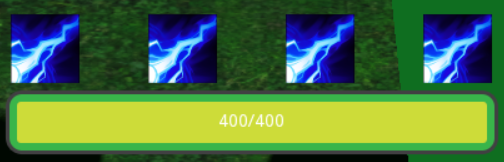
\includegraphics[width=0.6\linewidth]{figures/PlayerHUD}
	% \caption{Habilidades del personaje y barra de vida.}
	\label{fig:PlayerHUD}
\end{figure}

\vspace{\baselineskip}

\subsubsection{Match details}

En la parte superior de la pantalla se muestra el estado actual de los objetivos de la partida. La información mostrada variará según el modo del juego:

\begin{itemize}
	\item \textbf{Deathmatch}: Muestra el número de vidas restantes de cada equipo.
	\item \textbf{Captura}: Muestra la puntuación de cada equipo así como el tiempo de partida restante.
\end{itemize}

\begin{figure}[h]
	\centering
	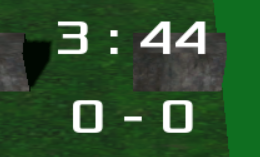
\includegraphics[width=0.6\linewidth]{figures/MatchDetails}
	% \caption{Match Details del modo de juego \emph{Captura}.}
	\label{fig:MatchDetails}
\end{figure}

	\newpage
\section{Personajes}

% ==============================================================================

\subsection{Ingeniera}

\textbf{Rol:} Daño a distancia

\begin{figure}[H]
	\centering
	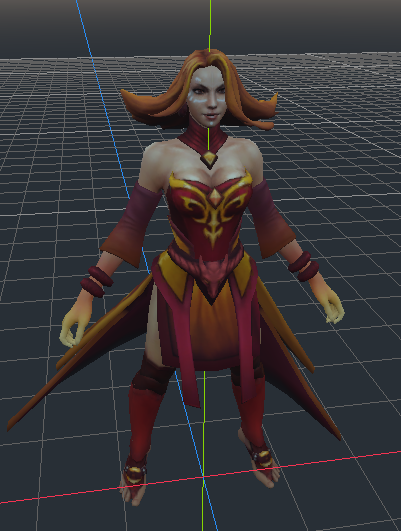
\includegraphics[width=0.4\linewidth]{figures/EngineerModel.png}
	% \caption{Ingeniera.}
	\label{fig:EngineerModel}
\end{figure}


La Ingeniera es un personaje que se especializa en el ataque a larga distancia mediante diversos tipos de proyectiles, aportando gran cantidad de daño a costa de tener poca vida y movilidad.

Para ser efectivo con ella, es importante mantener la distancia con los enemigos. Como la ingeniera solo tiene la $W$ para escapar del peligro, sus habilidades requieren que se quede inmóvil para usarlas y tiene poca vida, todo esto hace que sus opciones de supervivencia sean muy limitadas si los enemigos consiguen cubrir la distancia que los separa. 
% De esta forma, el gameplay de la ingeniera consiste en alejarse de los enemigos, atacarlos desde un lugar seguro y repetir este proceso cada vez que los enemigos consiguen acercarse.

\subsubsection{Habilidades}
\begin{itemize}
\item \textbf{Ataque Básico.} Dispara con una ballesta. El disparo hace poco daño pero tiene bastante rango. Es la única habilidad que no necesita que se quede quieta para usarse.
\item \textbf{Q.} Saca una pistola y dispara un proyectil de alcance infinito pero que no atraviesa obstáculos.
\item \textbf{W.} Dispara un gancho de alcance medio que, al impactar con un obstáculo, lleva a la ingeniera hasta este.
\item \textbf{E.} Dispara una granada que rebota con los obstáculos un número limitado de veces antes de explotar. 
% Tras chocar con un enemigo o alcanzarse el número máximo de rebotes, la granada explota, infringiendo daño en un área pequeña. 
El número máximo de granadas que puede haber en un momento dado en el mapa es de 3.
\item \textbf{Ultimate (R).} Saca una pistola gigante que tiene un tiempo de carga de 4 segundos antes de poderse usar. La pistola permite realizar 10 disparos en rápida sucesión con alcance ilimitado y que atraviesan todos los obstáculos y enemigos, causando daño moderado. Mientras la habilidad esté activa, la Ingeniera no puede realizar otra acción, pero la habilidad se puede cancelar en cualquier momento.
% Durante todo el proceso que dure la habilidad, la ingeniera no puede moverse del sitio. Si recibe crowd control (CC) durante el tiempo de carga o de uso de la habilidad, la habilidad se cancela, con lo que puede volver a moverse. También puede elegir cancelar la habilidad en cualquier momento de carga o uso. Al cancelarse, la carga de la ulti vuelve a 0. Esta habilidad tiene un CD largo.
\end{itemize}

% --------------------------------------------------------------

\subsection{Mago}
\textbf{Rol:} Apoyo / Tanque

\begin{figure}[H]
	\centering
	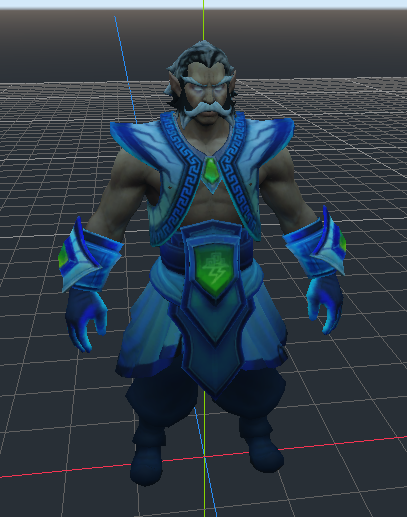
\includegraphics[width=0.4\linewidth]{figures/MageModel.png}
	% \caption{Mago}
	\label{fig:MageModel}
\end{figure}


El mago es un personaje de apoyo que se especializa en el control del mapa, proporcionando protección a su aliado y evitando que los enemigos puedan llegar hasta él. Sus características de \emph{tanque} le permiten preocuparse menos por su seguridad centrándose casi por completo en mantener a su aliado vivo y en darle apoyo.

Sus habilidades giran entorno al control del mapa y al posicionamiento de los distintos jugadores: él, su aliado y el equipo enemigo. Debe mantener alejado a su aliado del equipo enemigo, de ahí que tenga especial sinergia con campeones frágiles y/o con poca movilidad que tienen ataques a larga distancia. Su posicionamiento, en cambio, debe ser totalmente opuesto. Debido a sus habilidades y a su gran aguante, debe intentar siempre ``estar en medio'' del equipo enemigo, molestándolos e impidiéndoles llegar hasta su aliado.

\subsubsection{Habilidades}
\begin{itemize}
\item \textbf{Ataque Básico.} Da un golpe con su bastón. Este ataque, de corto alcance, hace muy poco daño pero invoca al hielo para aplicar una ralentización pequeña durante un periodo de tiempo.
\item \textbf{Q.} Invoca un elemento al azar sobre una zona. Los enemigos que pasen sobre esa zona recibirán un debuff que dependerá del tipo de elemento. De la misma forma, los proyectiles aliados que pasen sobre esa zona aplicarán el mismo debuff al impactar. Los elementos y sus debuffs asociados son: hielo - ralentización, fuego - daño por segundo, veneno - vulnerabilidad (aumenta el daño recibido por los siguientes ataques).
\item \textbf{W.} Intercambia su posición por la de su aliado.
\item \textbf{E.} Levanta un muro de piedra en la posición deseada.
\item \textbf{Ultimate (R).} Tras un largo tiempo de casteo (no cancelable) invoca a una tormenta que \emph{stunea} durante 5 segundos a los enemigos en una zona alrededor suya.
\end{itemize}

\newpage
	\section{Modos de juego}

\subsection{DeathMatch}
\emph{DeathMatch} se ubica en un pequeño mapa simétrico que enfrenta a los dos equipos en un continuo enfrentamiento, donde el objetivo es matar a los oponentes 5 veces.

\begin{figure}[H]
	\centering
	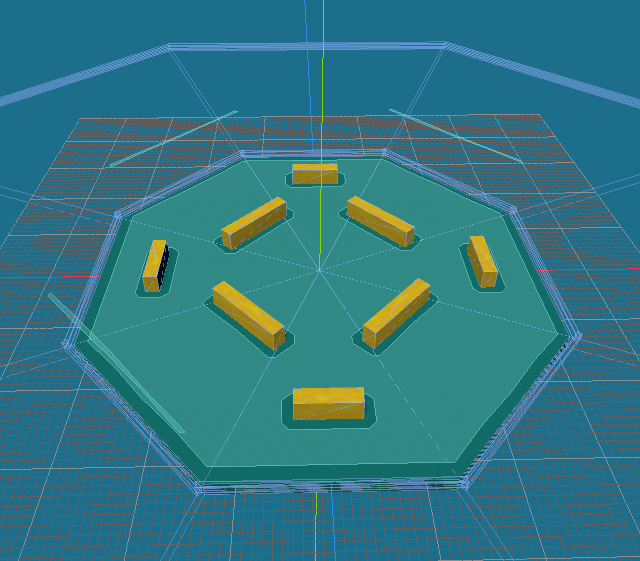
\includegraphics[width=0.5\linewidth]{figures/DeathMatchStage.png}
	% \caption{Escenario para el modo de juego DeathMatch.}
	\label{fig:DeathMatchStage}
\end{figure}

\vspace{\baselineskip}

\subsection{Captura}
Mapa grande donde los jugadores deben defender la zona del hada (la cual se va desplazando continuamente) el mayor tiempo posible. Los equipos reciben puntos por cada jugador que esté dentro de la zona en cada instante de tiempo. Una vez que han pasado 5 minutos, el equipo con más puntos gana.

\vspace{\baselineskip}

El mapa tiene tres tipos de zonas: la fortaleza central, las fortalezas de las esquinas y las zonas \emph{de paso}. Las fortalezas de las esquinas son fáciles de defender, al tener solo dos aperturas. La fortaleza central es más difícil de defender, al tener cuatro aperturas. Las zonas \emph{de paso} son zonas abiertas por las que se mueve el hada de una fortaleza a otra.

\begin{figure}[H]
	\centering
	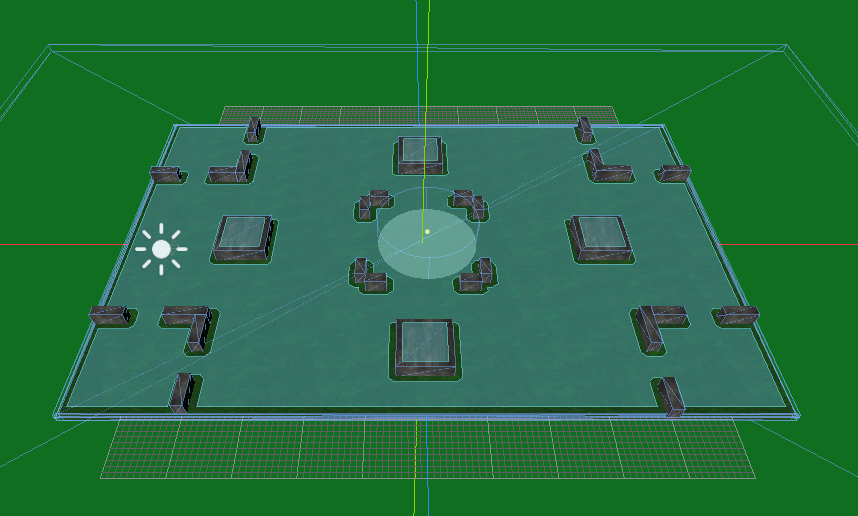
\includegraphics[width=0.7\linewidth]{figures/CaptureStage.png}
	% \caption{Escenario para el modo de juego Captura.}
	\label{fig:CaptureStage}
\end{figure}
	\section{Menús}

\subsection{Menú principal}
Esta es el menú que ve el jugador cuando abre el juego. Desde él se puede modificar el nombre (que se mostrará en partida), elegir el personaje a jugar en la siguiente partida, buscar partida, ver información sobre los personajes y cambiar las opciones de sonido.

\vspace{\baselineskip}

\begin{figure}[H]
	\centering
	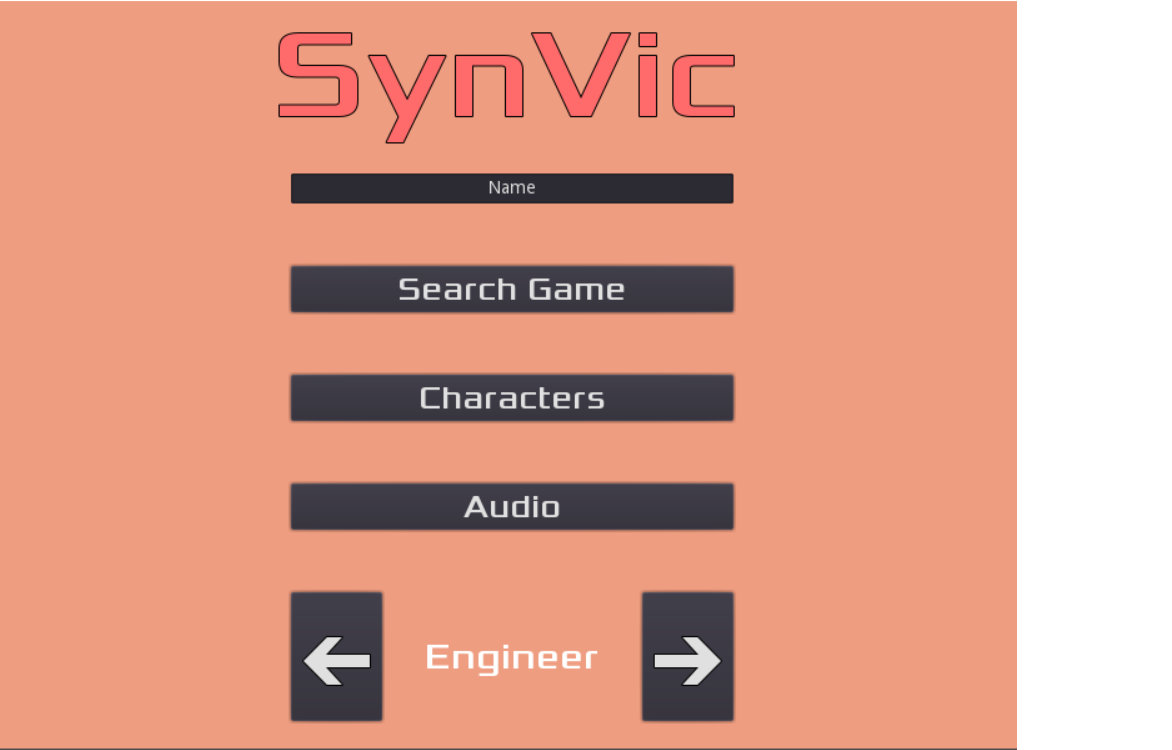
\includegraphics[width=0.7\linewidth]{figures/MainMenu}
	% \caption{Menú principal del juego.}
	\label{fig:MainMenu}
\end{figure}

\vspace{\baselineskip}
\vspace{\baselineskip}

\subsection{Menú de Sonido}
Permite configurar de forma separada el volumen maestro (que afecta a todo el sonido del juego), el volumen de la música y el volumen de los efectos de sonido. Además, se puede directamente silenciar cada uno de estos volúmenes por separado.

\vspace{\baselineskip}

\begin{figure}[H]
	\centering
	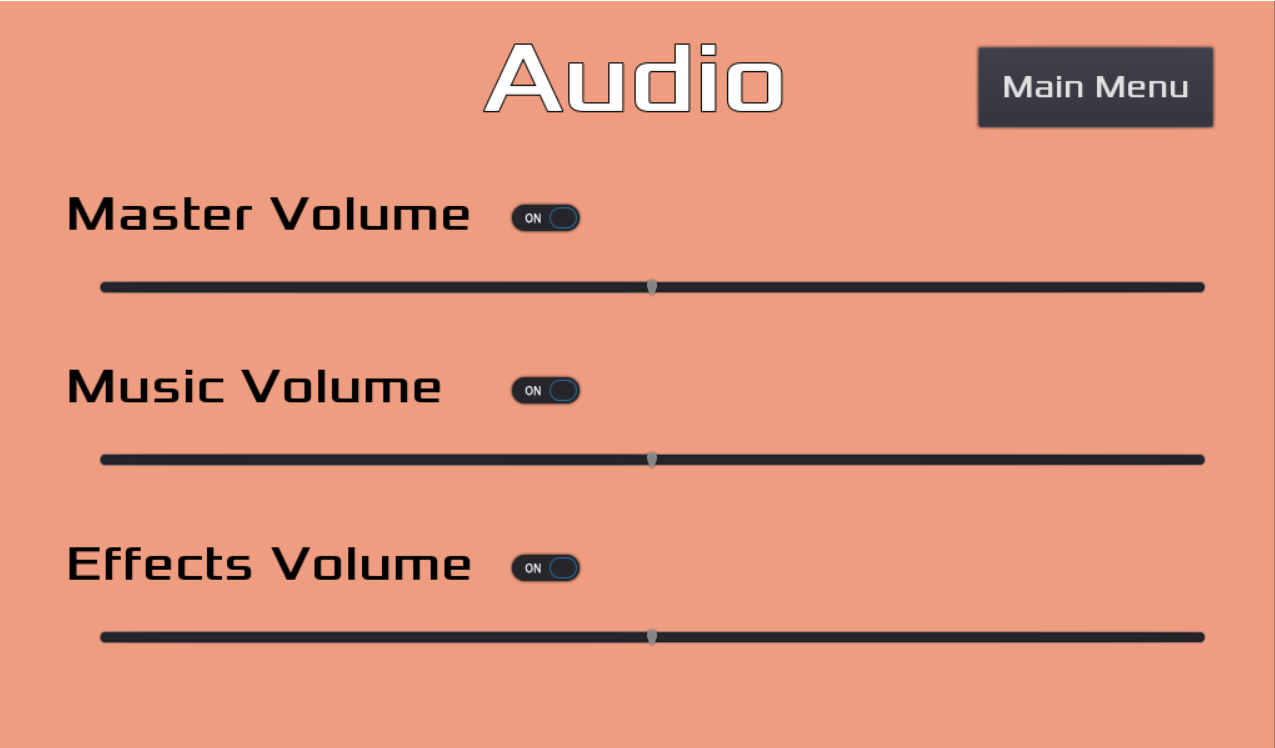
\includegraphics[width=0.7\linewidth]{figures/AudioMenu}
	% \caption{Menú de configuración de sonido.}
	\label{fig:AudioMenu2}
\end{figure}

\newpage

\subsection{Menú de Personajes}
En este menú se puede acceder a la información sobre cualquier personaje, incluyendo el funcionamiento de sus habilidades.

\vspace{\baselineskip}

\begin{figure}[H]
	\centering
	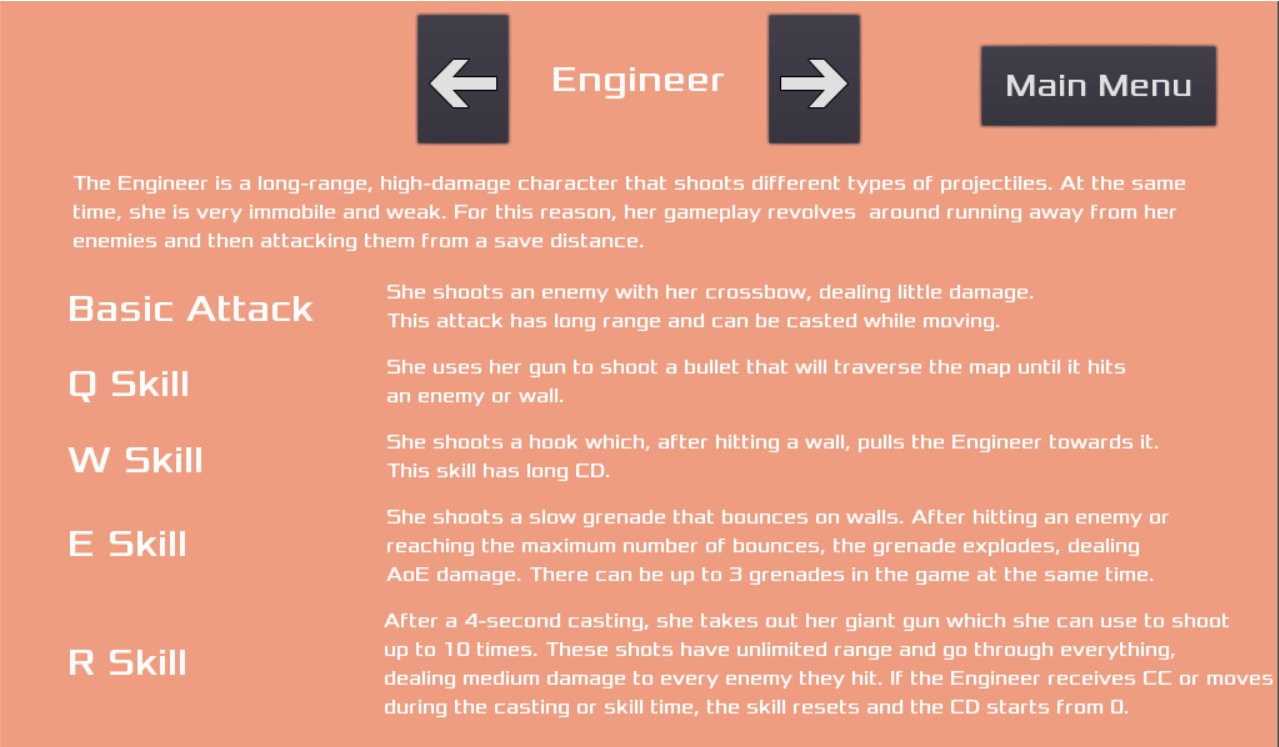
\includegraphics[width=0.7\linewidth]{figures/CharacterMenu}
	% \caption{Menú de personajes.}
	\label{fig:CharacterMenu}
\end{figure}

\vspace{\baselineskip}
\vspace{\baselineskip}

\subsection{Lobby}
Tras encontrar una partida, se accede al Lobby junto a otros tres jugadores. En el Lobby se muestra el tipo de partida (mapa) a jugar y se votan para elegir equipos en función de los distintos personajes. Cada jugador puede votar (\emph{botón flecha arriba}) a otro jugador para que sea su compañero de equipo y a otro (\emph{botón X}) para que \textbf{no} sea su compañero de equipo. En función de esta votación, se forman los equipos.

\vspace{\baselineskip}

\begin{figure}[H]
	\centering
	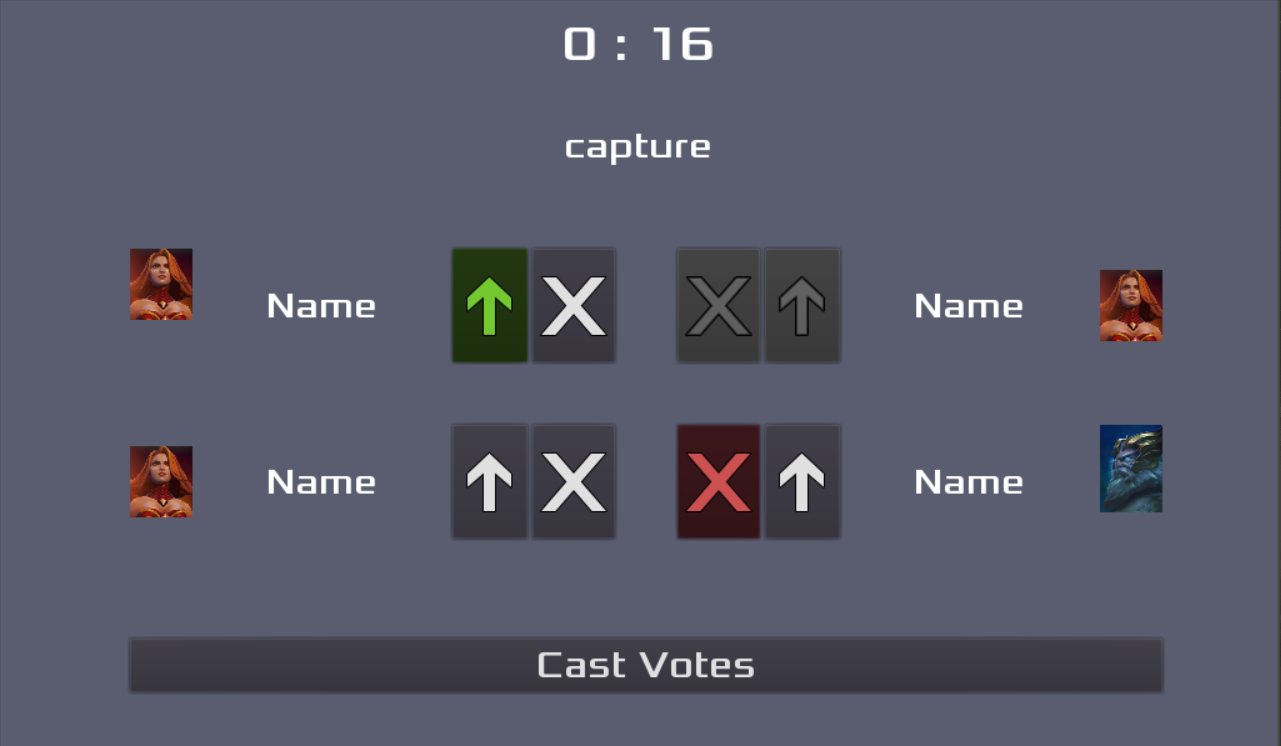
\includegraphics[width=0.7\linewidth]{figures/Lobby}
	% \caption{Lobby.}
	\label{fig:Lobby}
\end{figure}

    \setlength{\parskip}{1em}
    
    % ==============================================================================
\end{document}


\end{document}